\documentclass{article}
\usepackage{Sweave}
\usepackage{amsmath}
\usepackage{amscd}
\usepackage[tableposition=top]{caption}
\usepackage{ifthen}
\usepackage[utf8]{inputenc}
\usepackage{hyperref}
\usepackage[usenames]{color}
\definecolor{midnightblue}{rgb}{0.098,0.098,0.439}
\DefineVerbatimEnvironment{Sinput}{Verbatim}{xleftmargin=2em, fontshape=sl,formatcom=\color{midnightblue}}
\DefineVerbatimEnvironment{Soutput}{Verbatim}{xleftmargin=2em}
\DefineVerbatimEnvironment{Scode}{Verbatim}{xleftmargin=2em}
\fvset{listparameters={\setlength{\topsep}{0pt}}}
\renewenvironment{Schunk}{\vspace{\topsep}}{\vspace{\topsep}}

\begin{document}
\title{Assigning a p-value to consensusDistance in the Pathprint package}
\author{Gabriel Altschuler}
\maketitle
In considering the distribution of distances from a consensus fingerprint, a major problem is how to assign a measure of significance. This is particularly important if it is necessary to impose a cutoff at which to evaluate retrieved results. Calculating significance based on the distribution of fingerprint scores across the full GEO corpus is complicated as a) each pathway has a different distribution of ternary scores and b) the pathways scores are known to be correlated. An alternative strategy is to use the distribution of the corpus to define a background distribution, based on the following crude assumptions.
\begin{itemize}
\item The scores distribution is composed of two distinct populations; phenotypically matched and non-matched samples.
\item The distances of the non-matched samples are normally distributed.
\item The number of true phenotypicaly matched samples is negligible relative to the size of the corpus.
\end{itemize}
Thus, a p-value associated with a given distance can be calculated using the distribution function of N($\mu$, $\sigma$) where $\mu$ and $\sigma$ are the mean and standard deviation of the distances of all arrays in the fingerprint database. However, often the third assumption is not valid and the distribution is skewed. In this case, the estimated $\mu$ and $\sigma$ for the non-matched samples are not appropriate. To account for this an alternative is to use a trimmed mean to estimate $\mu$ and the inter-quartile range to estimate $\sigma$.
\section{Model data}
We can demonstrate the issue using a model dataset, composed of two independent normal distributions.
\begin{Schunk}
\begin{Sinput}
> pnorm.trim<-function(x, ...){
 # function to estimate a fit to the normal
 # distribution based on the interquartile range
   mean.trim.q <- mean(x, trim = 0.25)
  	IQR<-quantile(x, 0.75) - quantile(x, 0.25)
  	sd.trim.q<-IQR/(2*qnorm(0.75))	
  	pnorm(x, mean = mean.trim.q, sd = sd.trim.q, ...)
  	}
\end{Sinput}
\end{Schunk}
\begin{Schunk}
\begin{Sinput}
> x<-c(rnorm(1000, 20,5), rnorm(100,2,1))
> background.x<-
   dnorm(1:round(max(x)),
             mean = mean(x),
             sd = sd(x)
       )
> background.x.trim<-
   dnorm(1:round(max(x)),
             mean = mean(x, trim = 0.25),
             sd = (quantile(x, 0.75) - quantile(x, 0.25))/(2*qnorm(0.75))
       )
\end{Sinput}
\end{Schunk}
\begin{figure}
\begin{center}
\begin{Schunk}
\begin{Sinput}
> qqnorm(x)
> qqline(x, col = "red")
\end{Sinput}
\end{Schunk}
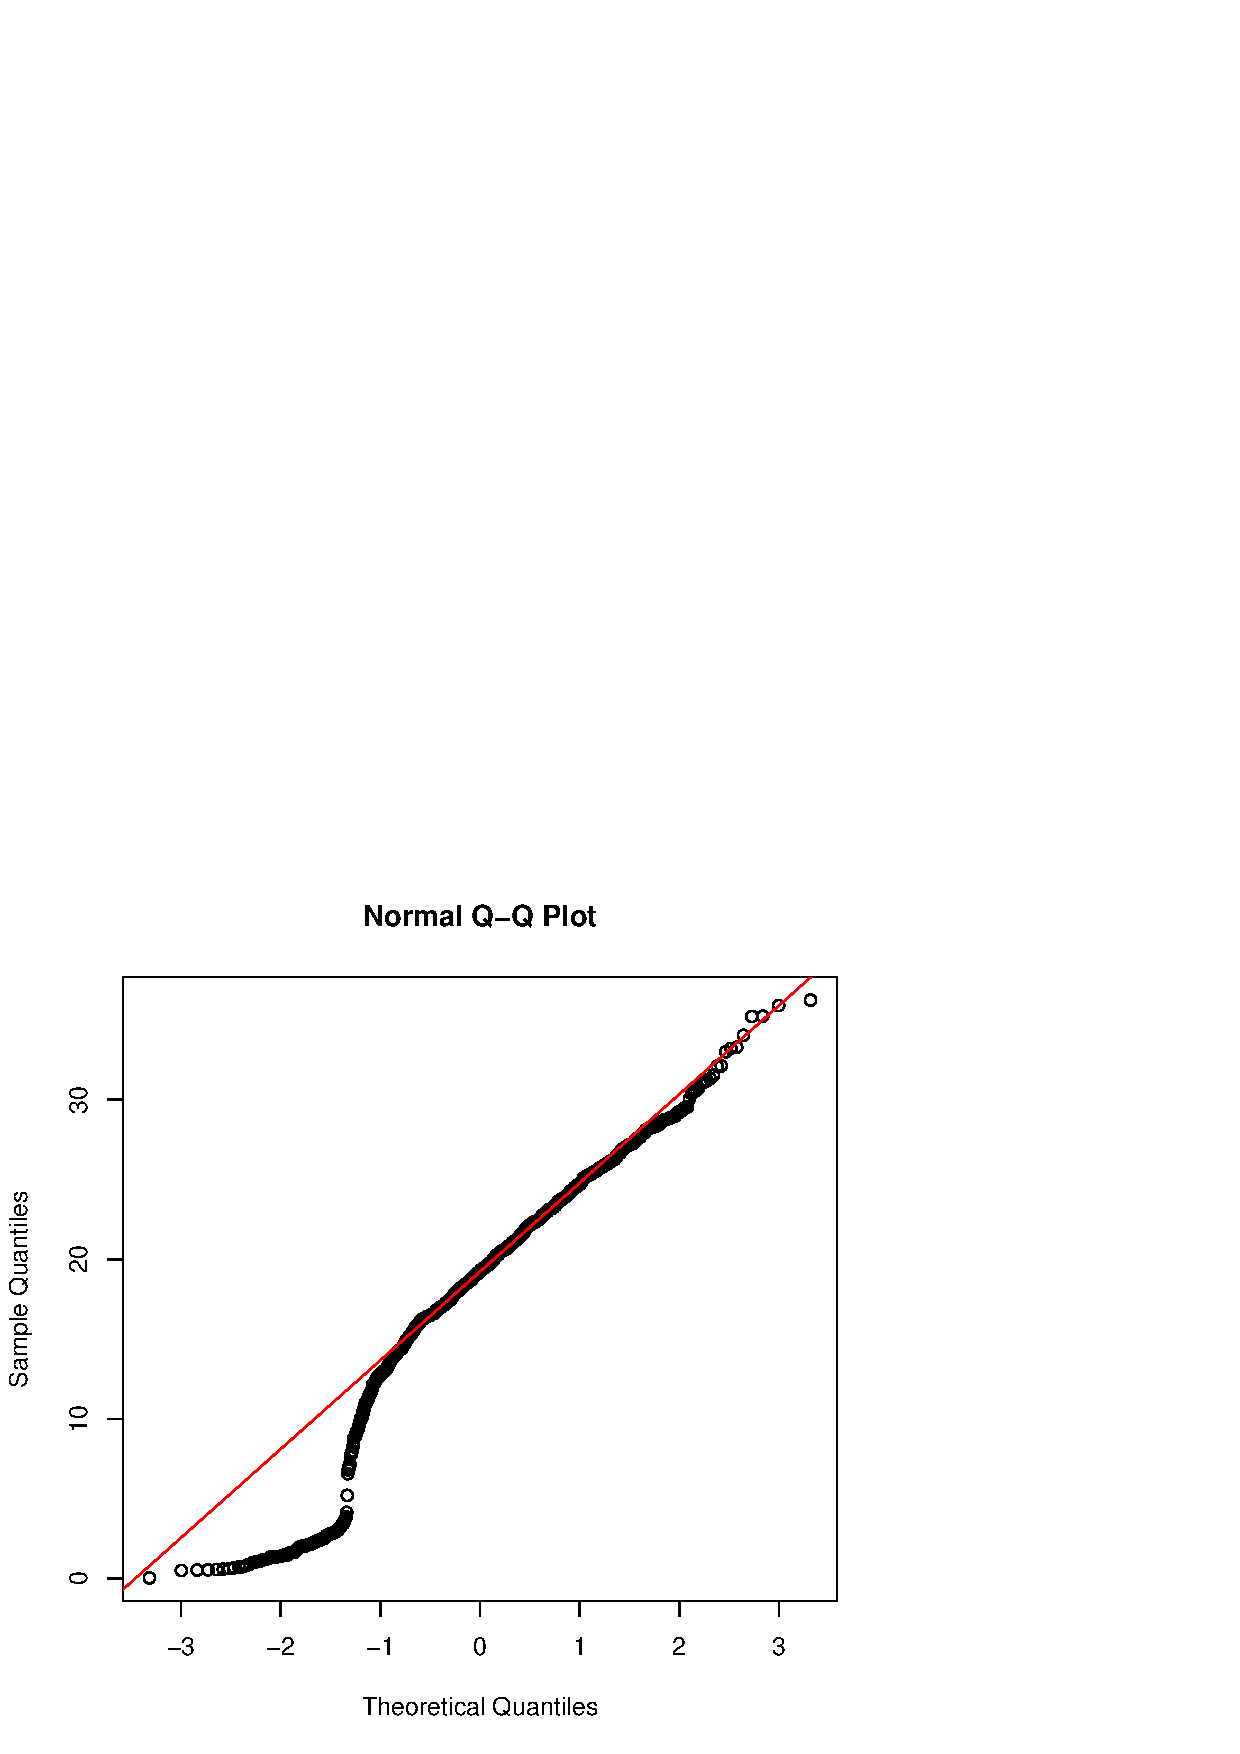
\includegraphics{figs/-qqplot}
\end{center}
\caption{Normal Q-Q plot for simulated bi-modal data, the red line passes through the first and third quartiles}
\label{fig:qqplot}
\end{figure}
A qqplot of the data, figure~\ref{fig:qqplot} demonstrates that data within the inter-quartile range is approximately normally distributed.
\begin{figure}
\begin{center}
\begin{Schunk}
\begin{Sinput}
> plot(density(x)$x, density(x)$y/max(density(x)$y), type = "l", xlab = "x", ylab = "Density or P-value")
> lines(background.x/max(background.x), col = "blue")
> lines(background.x.trim/max(background.x.trim), col = "red")            
> lines(x[order(x)], pnorm(x, mean(x), sd(x))[order(x)], col = "blue", lty = 2)
> lines(x[order(x)], pnorm.trim(x)[order(x)], col = "red", lty = 2)
> plot(density(x)$x, density(x)$y/max(density(x)$y), type = "l", xlab = "x", ylab = "Density or P-value", log = "y")
> lines(background.x/max(background.x), col = "blue")
> lines(background.x.trim/max(background.x.trim), col = "red")            
> lines(x[order(x)], pnorm(x, mean(x), sd(x))[order(x)], col = "blue", lty = 2)
> lines(x[order(x)], pnorm.trim(x)[order(x)], col = "red", lty = 2)
\end{Sinput}
\end{Schunk}
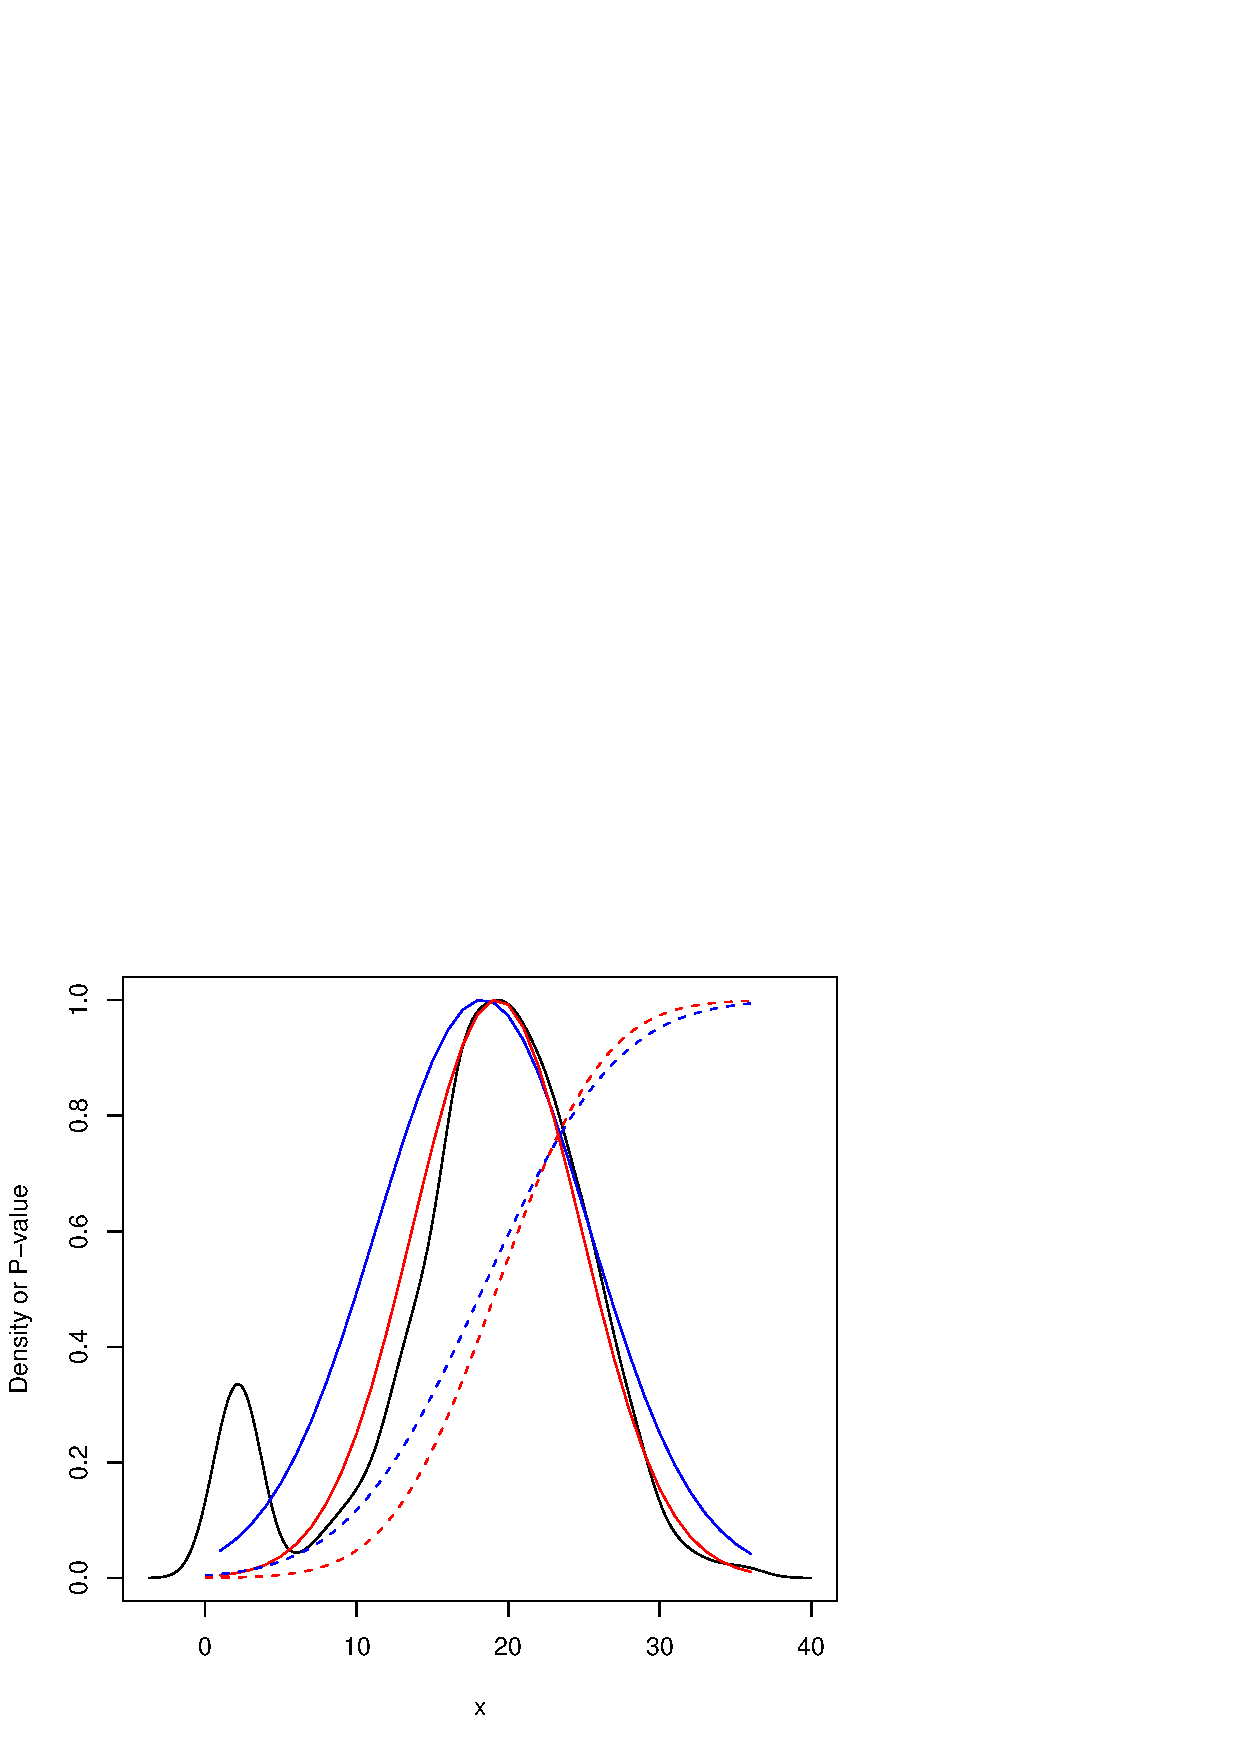
\includegraphics{figs/-distplot1}
\end{center}
\caption{Density plot for simulated bi-modal data, with background esitmation based on N($\mu$, $\sigma$) for the full data (blue) and the IQR (red). Dotted lines indicate p-values calculated based on these distributions, plotted with linear scale}
\label{fig:distplot1}
\end{figure}
\begin{figure}
\begin{center}
\begin{Schunk}
\begin{Sinput}
> plot(density(x)$x, density(x)$y/max(density(x)$y), type = "l", xlab = "x", ylab = "Density or P-value", log = "y")
> lines(background.x/max(background.x), col = "blue")
> lines(background.x.trim/max(background.x.trim), col = "red")            
> lines(x[order(x)], pnorm(x, mean(x), sd(x))[order(x)], col = "blue", lty = 2)
> lines(x[order(x)], pnorm.trim(x)[order(x)], col = "red", lty = 2)
\end{Sinput}
\end{Schunk}
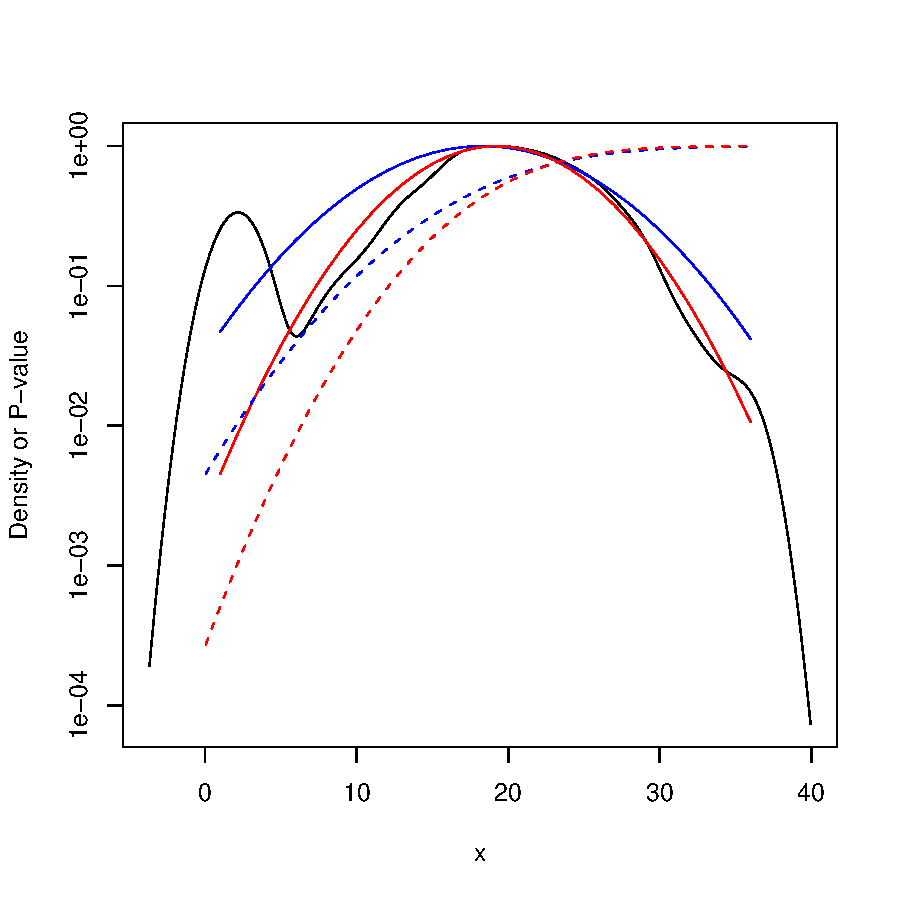
\includegraphics{figs/-distplot2}
\end{center}
\caption{Density plot for simulated bi-modal data, with background esitmation based on N($\mu$, $\sigma$) for the full data (blue) and the IQR (red). Dotted lines indicate p-values calculated based on these distributions, plotted with log scale}
\label{fig:distplot2}
\end{figure}

\end{document}

